\chapter{UI Design} \label{ch:ui_design}
The UI has been designed based on the model and function components, and with the client's wishes to have a functional and simplistic design, in mind. This approach is more functionality oriented, than making the UI and then basing the model and function components on that. The design has drawn inspiration from GitHub's desktop application and Overleaf's online LaTeX editor, as their designs are very simple and their color pallets are made up of low saturation colors. \par

The user interface has been designed based on a modern minimalistic design \citep{MinimalistUX} as this was a requirement from the client \autoref{sc:requirements}. This means that the design is flat and without a lot of shadows. Many of the corners in the application have been rounded for a milder look and the colors are very similar.

\section{Client feedback}
As mentioned above, the ideal UI, as described by the client, is simple and effective. This criteria has led to a UI with a limited set of colors, a cohesive design across the interface, and functionalities based on standards within the clients work environment, in this case Microsoft Windows. This is, for example, reflected in the way selecting elements in a list is similar to how it is done in Windows.
\par
Some things have been changed a bit from how they are handled in Windows, such as the before mentioned selection of elements in a list. On top of the standard Windows multi-selection, checkboxes have been implemented to make multi-select possible without holding down the 'Ctrl' key. The client can still use the basic Windows method, but will be able to take advantage of the checkboxes as well.

\subsection{Wireframes}
To ensure the compatibility between the clients workflow and the design, wireframes have been developed. Wireframes are an alternative to sketching designs on paper and then turning physical pages, as the user interacts with the system. The wireframes have been shown to the client in the early stages of the project to get feedback and improve the design, before starting coding functional prototypes.
\par
The wireframes have given a common basis for the further development of the system as well as the UI. One of the things that were illustrated in the wireframes was the page with the list of all assets in the system. This is one of the main pages of the system, as it will be used to access a specific asset, as well as search through, delete, edit, and print out a list of the assets. The wireframe is very simple and only uses black, white, and gray (see \autoref{fig:AssetList_Wireframe}).

\begin{figure}[H]
    \centering
    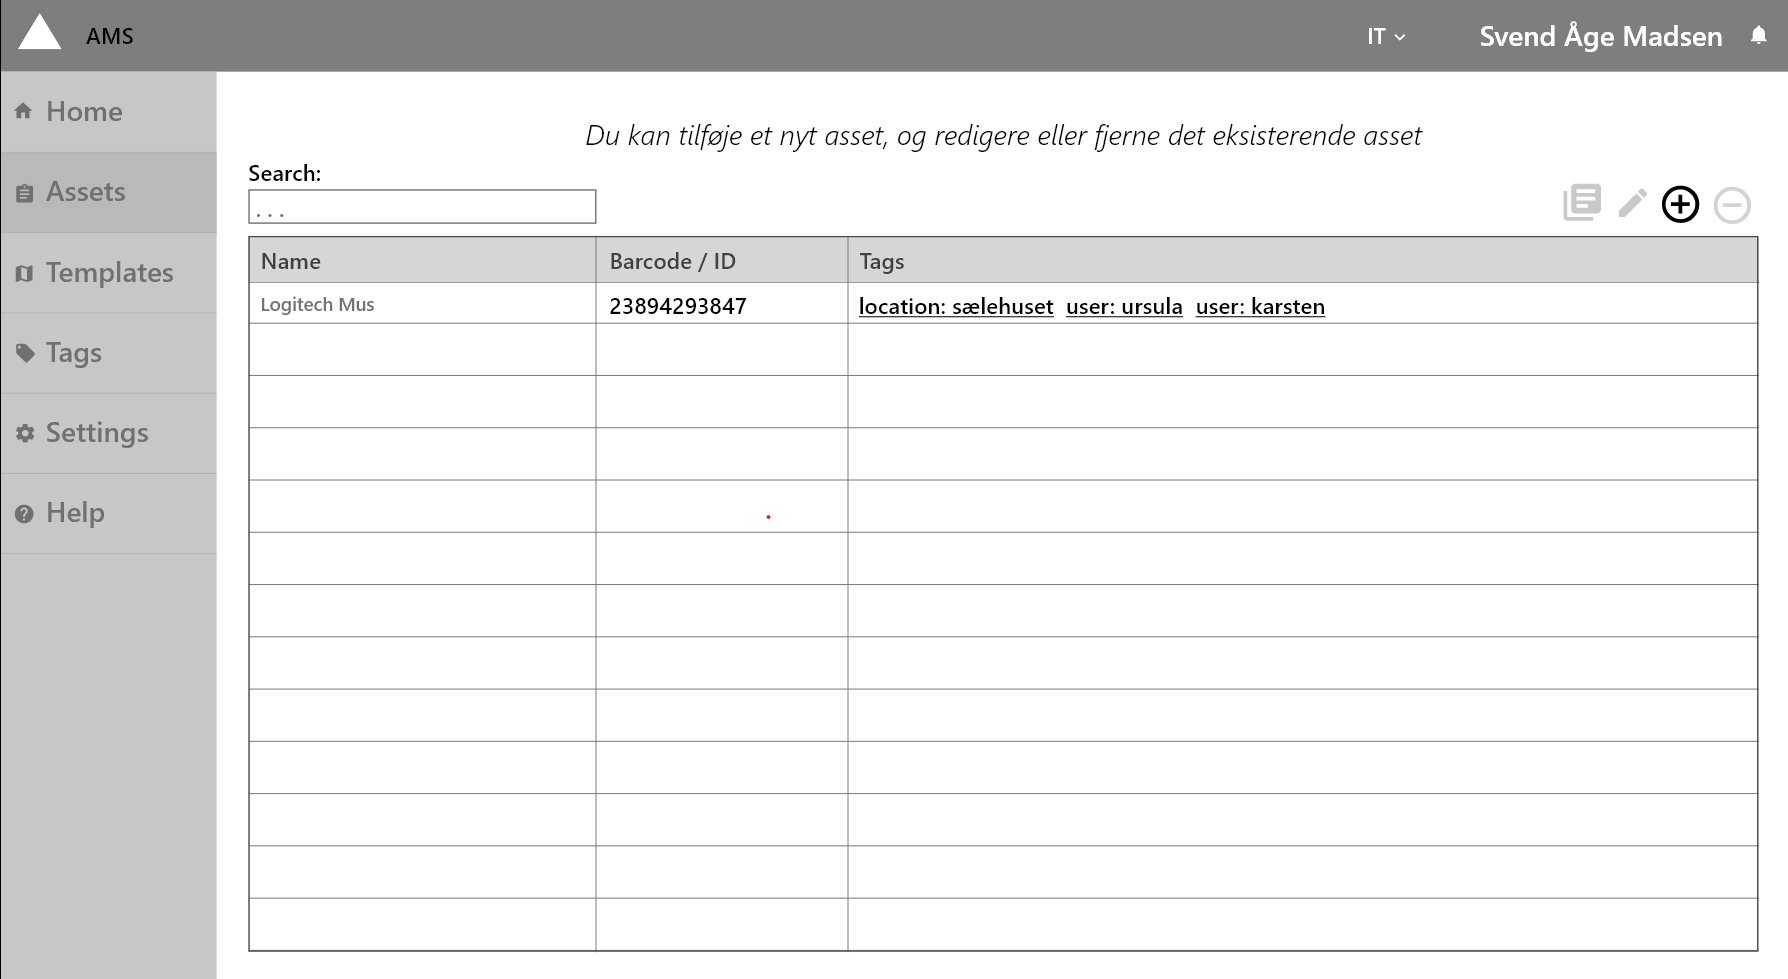
\includegraphics[width=0.8\textwidth]{figures/wireframes/AssetList_Wireframe.png}
    \caption{Wireframe of the AssetList page}
    \label{fig:AssetList_Wireframe}
\end{figure}

Another one of the essential pages is the one used for creating and editing an asset. This page has been illustrated with a few more elements than the list page, as it was important to show the client how it would look after an asset had been assigned several tags and fields. This was important, as the clutter \todo[inline]{reference to the place where we define the clutter as a problem} a lot of fields could result in, has been the reason for the client to get a custom system, instead of going with an already existing solution. 
\par
The dark grey header and side navigation are consistent across all pages, as they contain functionality that should be available to the user at all times. The asset editor page also contains a number of fields and attached tags, as this is another specific request from the client (see \autoref{fig:AssetEditor_Wireframe}).

\begin{figure}[H]
    \centering
    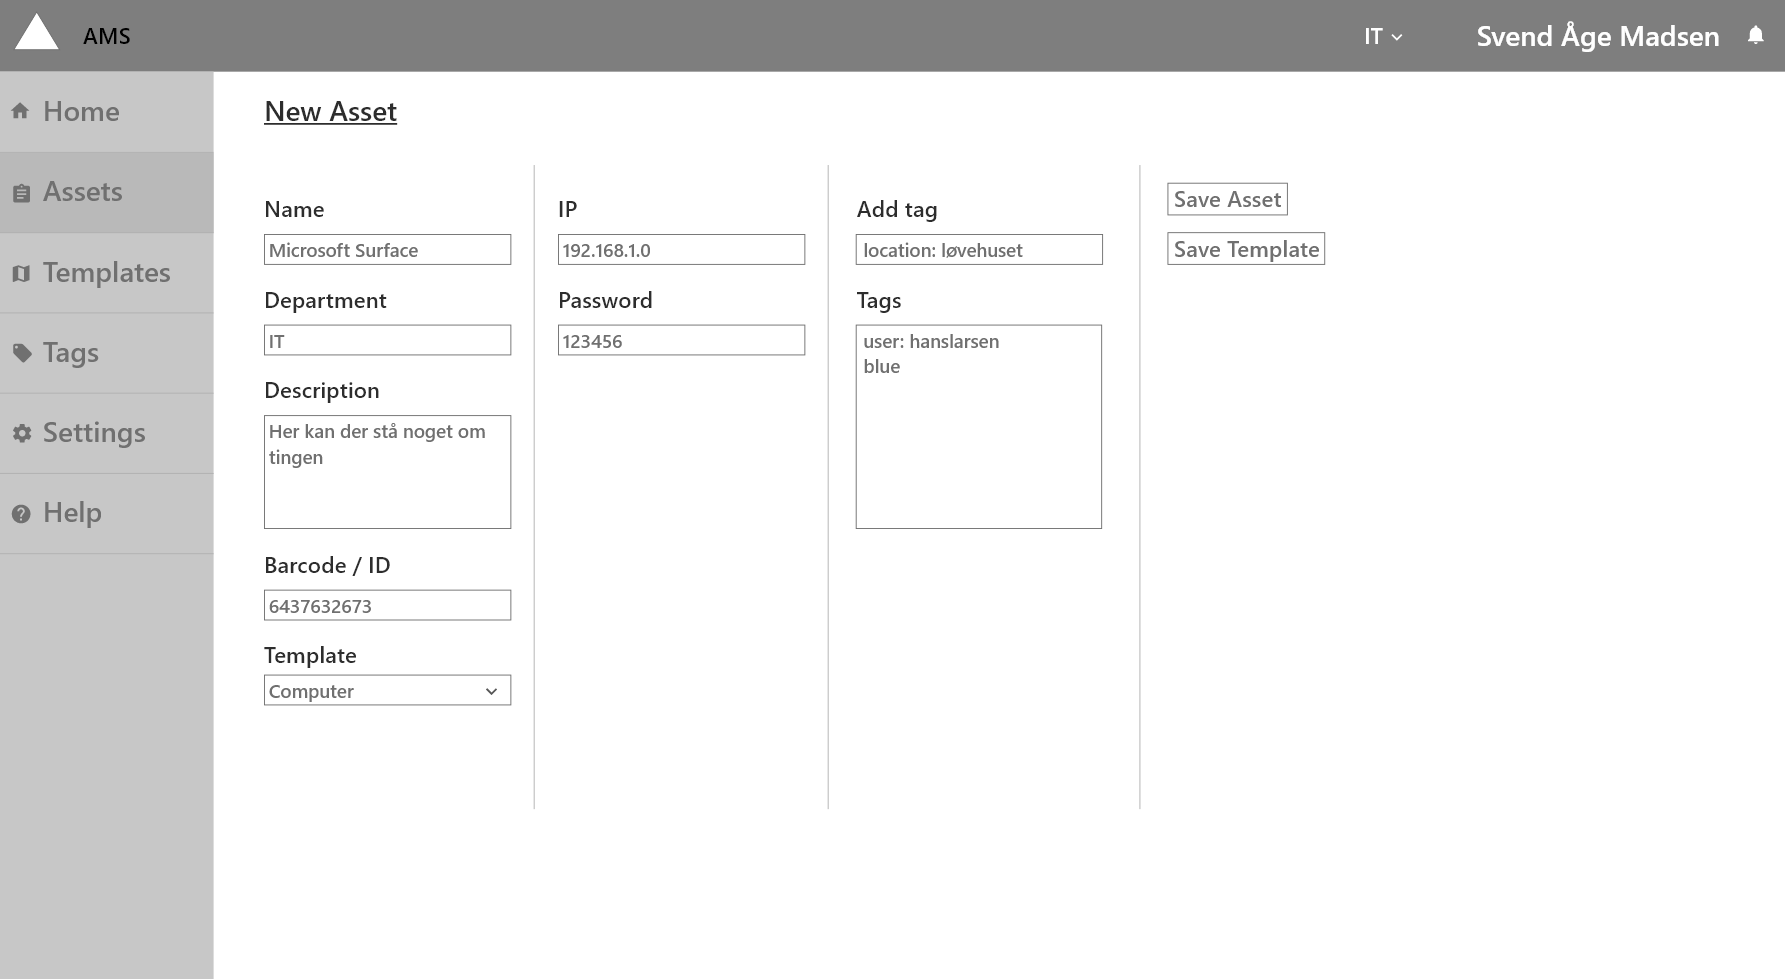
\includegraphics[width=0.8\textwidth]{figures/wireframes/AssetEditor_Wireframe.png}
    \caption{Wireframe of the AssetEditor page}
    \label{fig:AssetEditor_Wireframe}
\end{figure}

The wireframes were well received by the client, as they were very simple and had low saturation. The relatively few elements on the pages also followed the requirements from the client \autoref{sc:requirements}.

\subsection{Prototypes}
Based on the wireframes, multiple prototypes have been constructed to show the functionality in action. These prototypes include a visualization of the tagging of assets, which was written in Javascript (see \autoref{fig:PrototypeOfTagging}), as well as a limited, simple version of the system written in HTML, CSS, and Javascript (see \autoref{fig:PrototypeOfSystem}). This method of creating simple prototypes made it possible to show the client the system in a browser, as prototyping in HTML and Javascript is a faster way of creating a visual prototype.
\par

The problem with this method was that the code had to be written in both C\# and HTML and Javascript, and two different programming languages might have different limitations. The implementation of certain functions might therefore be more difficult in one language compared to another.
\par
The tagging prototype (see \autoref{fig:PrototypeOfTagging}) was important, as the experience of tagging has been hard to depict. This is primarily because a similar tagging system haven't been found in another system, and therefore had to be made from scratch. Because of this the main purpose of this prototype has been to understand how the client intended to use the functionality in the final product. Especially the keyboard shortcuts that the client tried to use to accomplish different actions, were noted for later implementation in the system. Actions such as entering a parent tag to attach the child tags, stepping out of the parent tag when pressing backspace without anything in the field, and how to show attached tags beneath the field.

\begin{figure}[H]
    \centering
    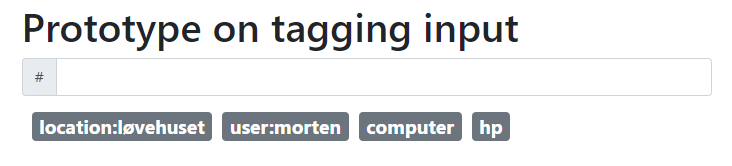
\includegraphics[width=0.8\textwidth]{figures/Prototypes/PrototypeOfTagging.png}
    \caption{Prototype of tagging}
    \label{fig:PrototypeOfTagging}
\end{figure}

The client had a few ideas related to the actions of different keyboard shortcuts, which were implemented in the final system. These include the suggestion list beneath the field, which automatically updates itself every time a key is pressed, as well as pressing the tab key to auto fill with the first element in the shown list.
\par
To accompany the prototype of the tagging, the client has been shown a prototype of the overall design of the system as well. This prototype was, as mentioned above, written in HTML, CSS, and Javascript and implemented some overall functions such as adding an asset, viewing the information of an asset, and adding fields to the asset. The prototype was not connected to a database and the actions were only for illustrative purposes with no actual effects. \autoref{fig:PrototypeOfSystem} depicts the page for editing an asset in the prototype.

\begin{figure}[H]
    \centering
    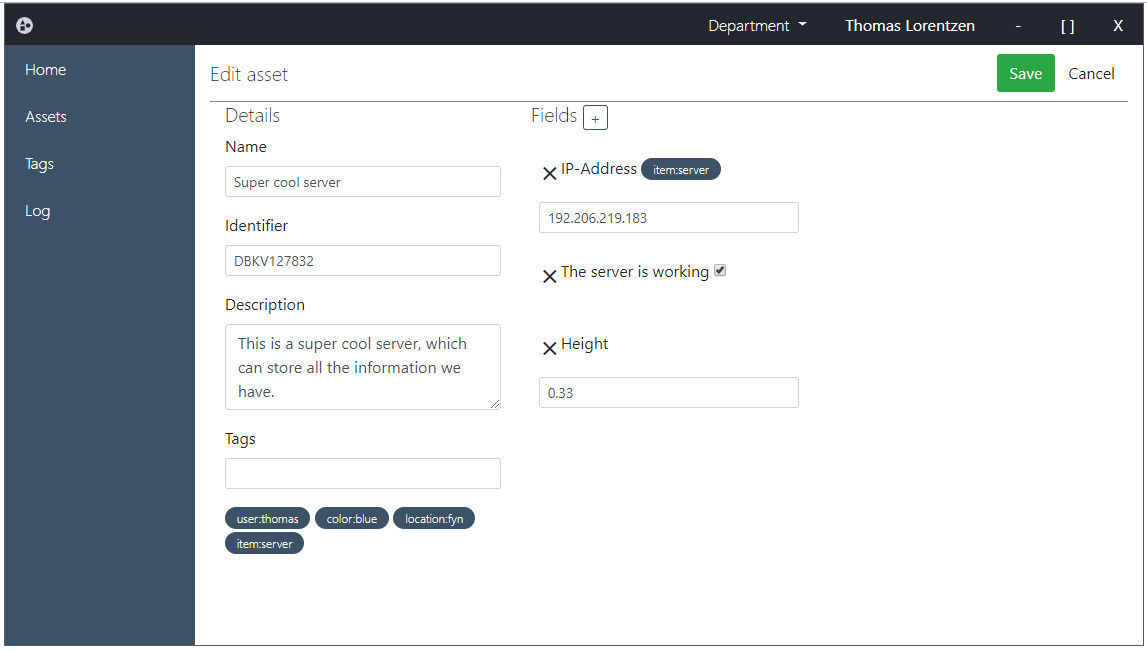
\includegraphics[width=0.8\textwidth]{figures/Prototypes/AssetEditor_Prototype.png}
    \caption{Prototype of system}
    \label{fig:PrototypeOfSystem}
\end{figure}

The client was very pleased with the designs of the prototypes and therefore they have been used as a basis for the final design.

\subsection{Early usability tests}
Based on the feedback from the wireframes and prototypes, the parts depicted in the wireframes and prototypes was developed. A usability test of the early version of the system was done with the client, before too many details and functionalities were implemented. This was done to ensure that the client agreed with the direction in which the functionality and design of the system was developed. 
\par
Another usability test was also performed on a participant with no previous knowledge of the system, but with experience within IT, in order to evaluate the usability of the design as a whole. This was done before the test with the client, which also provided some experience with doing usability tests before involving the client. A screenshot of the system during the usability tests can be seen below (\autoref{fig:UsabilityTestsEditAssetPage}).

\begin{figure}[H]
    \centering
    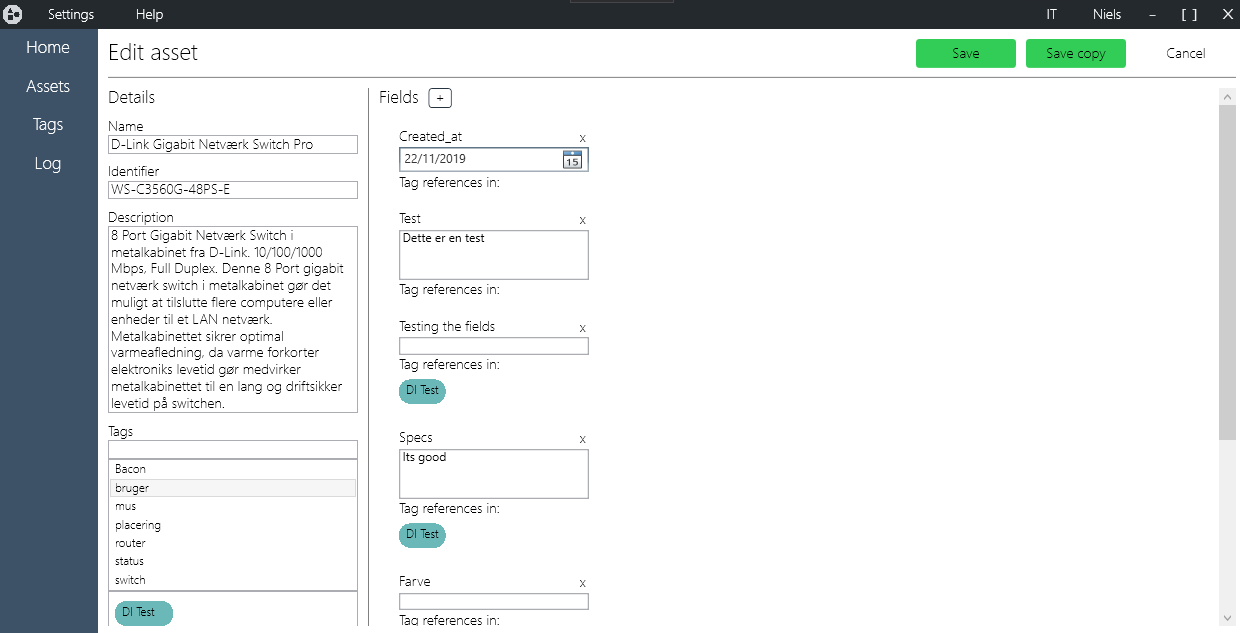
\includegraphics[width=0.8\textwidth]{figures/PicturesOfTheSystem/Usabilitytest_editAsset.png}
    \caption{A screen shot of the 'edit asset' page from the usability test}
    \label{fig:UsabilityTestsEditAssetPage}
\end{figure}

One of the things that became clear through the usability tests in the early stages of the system development, was that our participants' intuition, when asked to remove an asset from the system, was to navigate to the edit page of the specific asset and then delete it from there. As seen in \autoref{fig:UsabilityTestsEditAssetPage}, there is no button on the edit page that supports the functionality to remove the asset from there.\\
The system only supported removal of an asset from the list page (see \autoref{fig:UsabilityTestsAssetListPage}), but this was not as intuitive to the test participants. Therefore a 'Remove' button was added to the 'Edit asset' page in the final design (see \todo{Insert reference to finished system design of edit asset page}).

\begin{figure}[H]
    \centering
    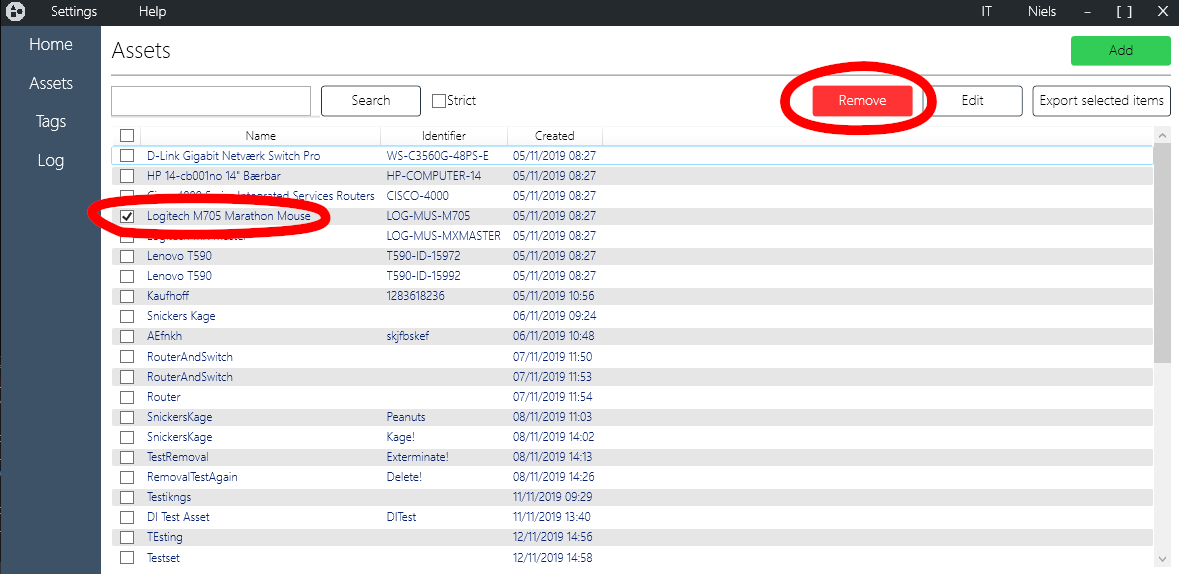
\includegraphics[width=0.8\textwidth]{figures/PicturesOfTheSystem/Usabilitytest_AssetList.png}
    \caption{A screenshot of the 'asset list' page from the usability test. The 'Remove' button is red, when the mouse is hovering over it, and is just black text when the mouse is not hovering over it.}
    \label{fig:UsabilityTestsAssetListPage}
\end{figure}

Multiple other functionalities and alterations to the design have been implemented in the final product based on the usability tests and the above example is only one of them.
\par
The client was again very pleased with the design of the interface, even though multiple functions had yet to be added and updated to better accommodate usability and the workflow of the client.

\section{Final design}
The final design of the user interface has been developed based on the feedback from the client and other usability test participants as well as the early sketches and prototypes.

\subsection{Overall concepts}
The UI has been designed with cohesion in mind to give the impression of a connected system. Some of the ways this has been achieved are through the color pallet, the simplicity across all the different pages, the left and top menu bars, the positions of buttons, and consistent fonts and font sizes.
\par
The UI has also been developed to be as intuitive to the client as possible. Achieving this has been difficult, but as the client is a Windows user with experience in different enterprise applications, the system implements as many shortcuts and functions native to the Windows platform as possible, in order to support the client's natural workflow.
\par
The design has also been developed in such a way that it accommodates the user's memory and attention span. This is visible in the way the user never needs to remember the previous steps when using the system. There are no pages, where the information from the previous page is crucial, and the tags make it possible to group similar assets, to make them easier to find through the search function on the list page. As well as making it easier to create similar Assets.
\par
The interface accommodates the attention span of the user by making it possible to save progress and return to the task later, in most of the scenarios. This is important, as the user might be distracted during their interactions with the system.
\par
Some of the areas of the design have been described in further detail below.

\subsubsection*{Navigation}
Navigating the system is very important, as the system supports a few different elements, which are handled on different pages. To make the navigation faster and more intuitive to the client, the left menu bar is visible from anywhere within the application. Through this, the pages for the different elements are accessible. The navigation bar also ensures that each page is at most three clicks away from anywhere within the application (see \autoref{fig:UIStructure}).
\par
For example if the user wants to see a specific asset, they press the 'Assets' tab in the navigation menu which will take them to the 'Asset list' page. From here they can remove assets, or access the 'View' or 'Edit' pages for every asset. If the asset is too far down the list or difficult to find, the user can use the search bar to find the asset.

\begin{figure}[H]
    \centering
    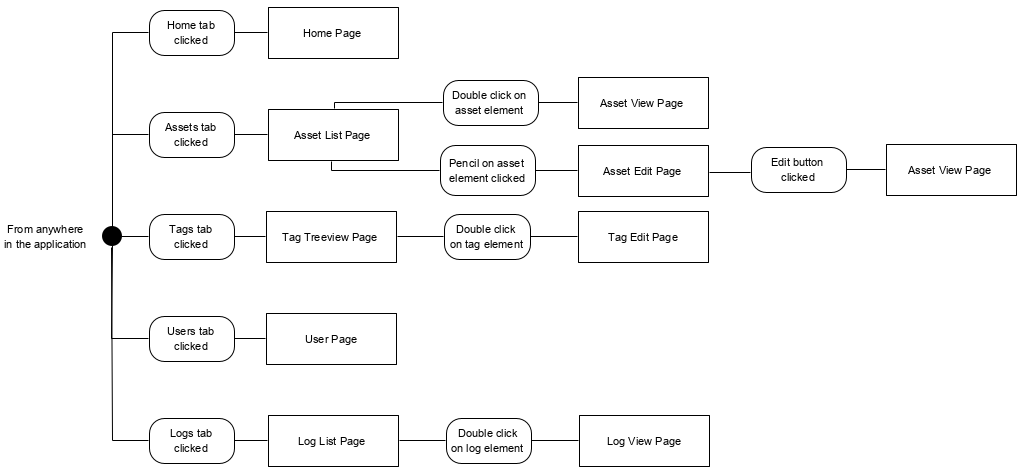
\includegraphics[width=1\textwidth]{figures/UIDesignElements/UI_Design_Structure.png}
    \caption{Diagram of the navigation structure of the system}
    \label{fig:UIStructure}
\end{figure}
\todo{Shortcuts?}

Besides this, navigating to the subpages, such as the 'View asset' page, is possible in multiple ways. When the user wants to view an asset, they can double click the asset in the list, press the eye symbol in the right side of the list element, or select it and then press either 'Enter' or 'Ctrl' + 'W'. This gives the user the ability to navigate the interface in a way that is intuitive to them.
\par
Because of the limited number of steps between the different pages, the only type of breadcrumb implemented is the highlighting of the page on the side bar that the user is currently on. If the page layout had multiple steps, a location-based page hierarchy \citep{Breadcrumbs} could be shown in the top of the window.

\subsection{Design methods}
In the design of the UI, a few different design methods and theories have been used. The usage of some of these have been described below.

\subsubsection*{Color}
The color pallet was heavily inspired by the GitHub desktop application and the Overleaf LaTeX editor \citep{GithubDesktop}\todo[inline]{Reference til Overleaf}. The inspirations have been drawn in order to save time on color selections for every part of the system, and these specific examples have been chosen due to their low saturation and very mild color pallet.

\begin{figure}[H]
    \centering
    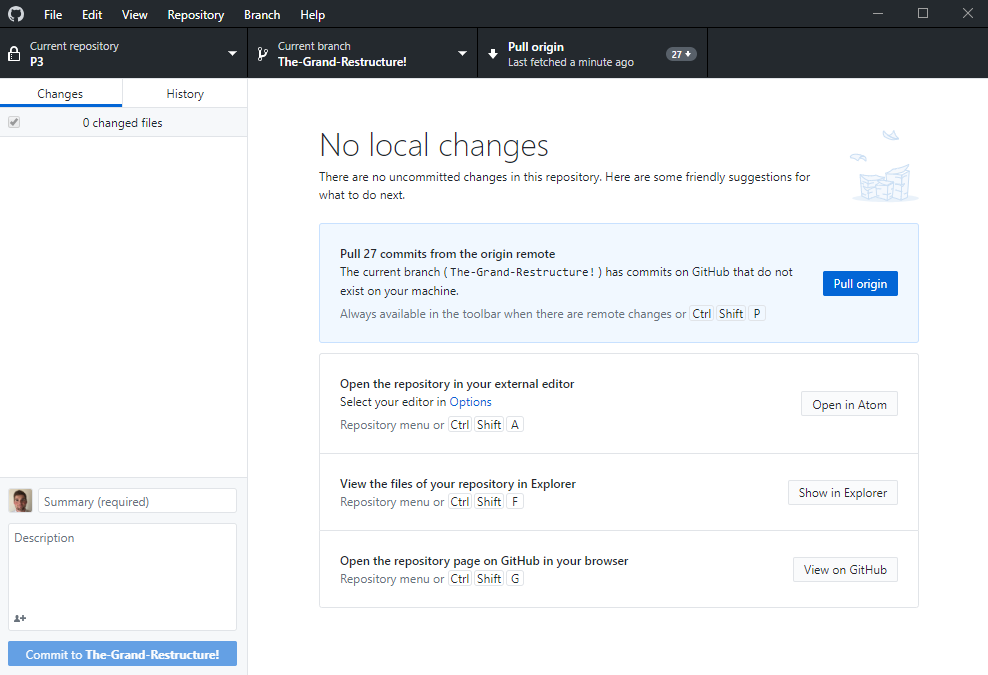
\includegraphics[width=0.8\textwidth]{figures/UIDesignElements/GitHub_Desktop_Screenshot.png}
    \caption{Screenshot of the GitHub desktop application \citep{GithubDesktop}}
    \label{fig:GitHubDesktop}
\end{figure}

For the buttons of the application, the dark border and white center was chosen for buttons that did not need to draw a lot of attention. The border is to illustrate the boundaries of the buttons.
\par
When the user hovers over any of the buttons in the application, the color changes to the color of the top menu bar \todo[inline]{Med untagelse af remove knapperne?}. This gives the user clarity about whether or not the button is clickable and that the cursor is pointing at it (see \autoref{fig:HoverColorAndBorderedButtons}).

\begin{figure}[H]
    \centering
    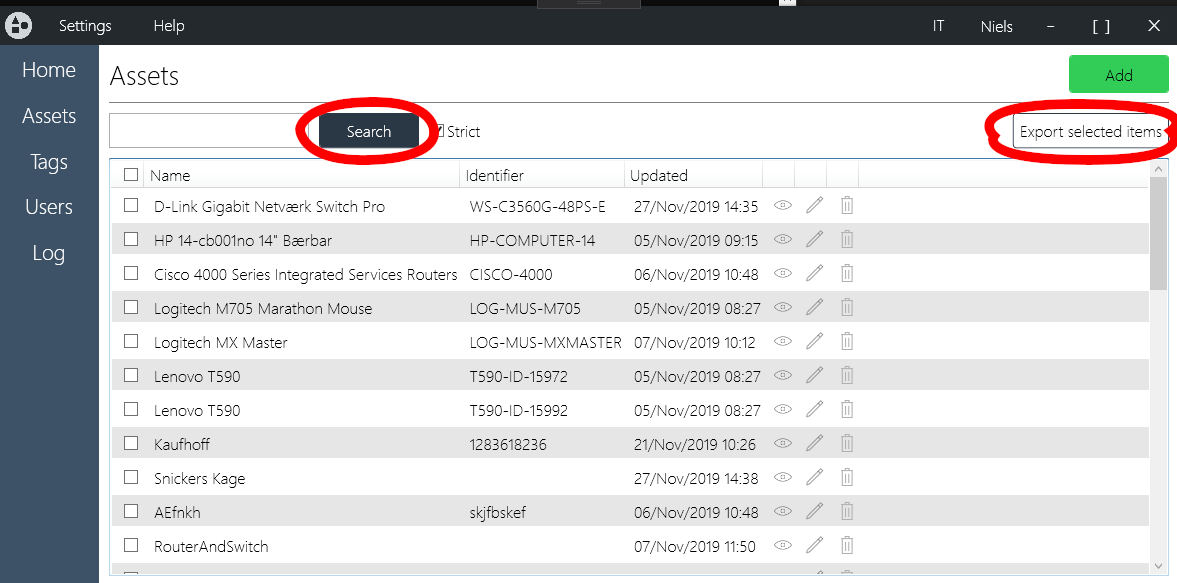
\includegraphics[width=0.8\textwidth]{figures/UIDesignElements/ButtonColors_AssetList.png}
    \caption{Screenshot of the 'Asset List' page, with the mouse hovering over the 'Search' button and not the 'Export selected items'}
    \label{fig:HoverColorAndBorderedButtons}
\end{figure}

The 'Add', 'Remove', and 'Delete' buttons and icons have been colored green and red respectively. This is because the red color signifies danger and alarm, and the green color signifies additions and improvement.

\subsubsection*{Gestalt Laws}
Buttons and other elements in the design have been implemented and placed in correlation with the Gestalt laws \citep{GestaltLaws}. This can be seen throughout the application, such as the way the search bar and 'Search' button are located right next to each other, to symbolize a connection between them (see \autoref{fig:UsabilityTestsAssetListPage}). Another example of the Gestalt laws, are the elements in the different lists in the application. The way that every other element is another color gives the experience of connection between the different columns in each row (see \autoref{fig:ChangingRowColors}).

\begin{figure}[H]
    \centering
    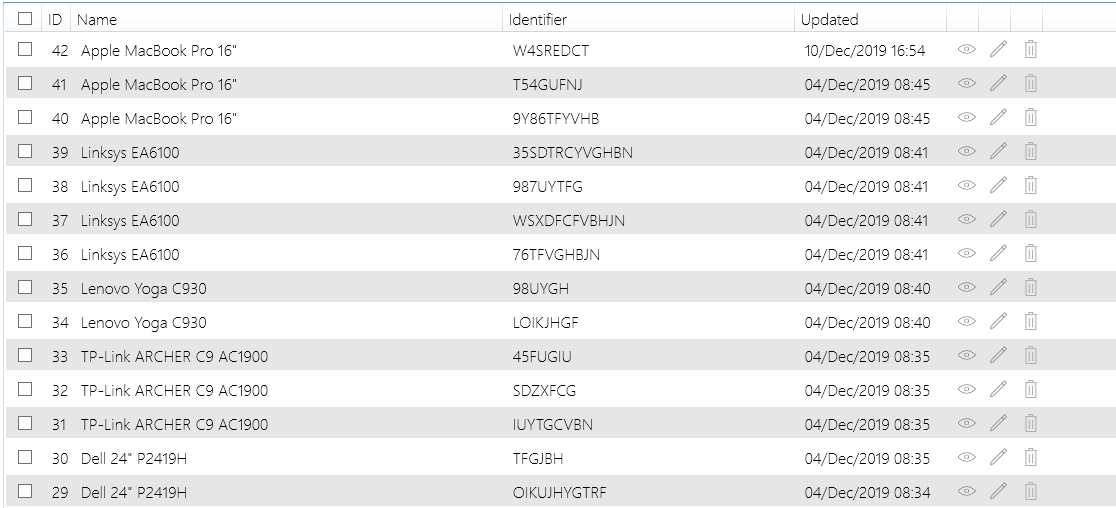
\includegraphics[width=0.8\textwidth]{figures/UIDesignElements/DifferentColoredRows.png}
    \caption{Screenshot of the rows in the 'Asset list' page}
    \label{fig:ChangingRowColors}
\end{figure}

These are some of the elements in the system that have been created with the Gestalt laws in mind.

\subsubsection*{Notifications}
During a normal interaction period with the system, several things might happen that the user should be notified of. These things include the results of interactions with the system that can be hard to understand the effects of, such as saving an asset, where the user is simply sent to another page. \\
Another thing that the user should be notified about, is limitations, such as not being able to edit multiple assets at a time. To give the user a clarity regarding these things, notifications are shown in the top of the application window.
\par
Notifications have different meanings and causes, and therefore they are given different colors as well. Notifications about operations succeeding are green, failed ones are red, and one with other information are yellow (see \autoref{fig:AssetAddedNotification}). These colors are derived from how other applications color notifications and the general understanding of how these colors are perceived.

\begin{figure}[H]
    \centering
    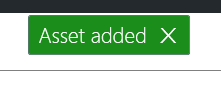
\includegraphics[width=0.4\textwidth]{figures/UIDesignElements/GreenNotification.png}
    \caption{Screenshot of the 'Asset added' notification}
    \label{fig:AssetAddedNotification}
\end{figure}

The notifications appear, as mentioned above, in the top of the screen and disappear after a few seconds. This is to avoid cluttering the interface with error messages. This could be a problem, if the notification disappears before the user sees it, but the notifications are designed only to hold a short text with information about the result of the previous operation or interaction with the system.

\section{Summary}
The design has, as mentioned in the above sections, been developed in close cooperation with the client and with focus on supporting their workflow and intuition. Further design elements and functions have been created as the needs and wants of the client were discovered.
\par
Through designing the UI, the Gestalt laws and other design philosophies have been implemented and used as reference to ensure a coherent and useful user-experience of the system, as well as keeping a minimalistic interface.
\todo{Insert picture of final design and possibly final usability test}